\glsresetall
\chapter{Proposed Solution}
\label{chap:proposed_solution}

In this Chapter, we present and discuss a possible solution to be implemented regarding the main problem to solve in this research, the data to process and the research questions to be answered. To present the solution and explain it, we will cover some aspects considered when defining a software based solution. This topics are: functional requirements~\ref{sec:functional_requirements}, quality attributes (non-functional requirements)~\ref{sec:quality_attributes} and finally, the architecture~\ref{sec:architecture} produced based on all previous topics.

The starting point for our proposed solution is the tracing data provided by Huawei. Tracing must be ingested by an entry component, capable of extracting metrics from tracing data. The outcome of this module are metrics and metadata in files to be further processed by a second component. This second component has the duty of analysing the output data from the first module, and point out service anomalies.

For a clear insight about our solution, the proposed approach in high level of abstraction is presented in the Figure~\ref{fig:proposed_approach}.

\begin{figure}[H]
    \centering
    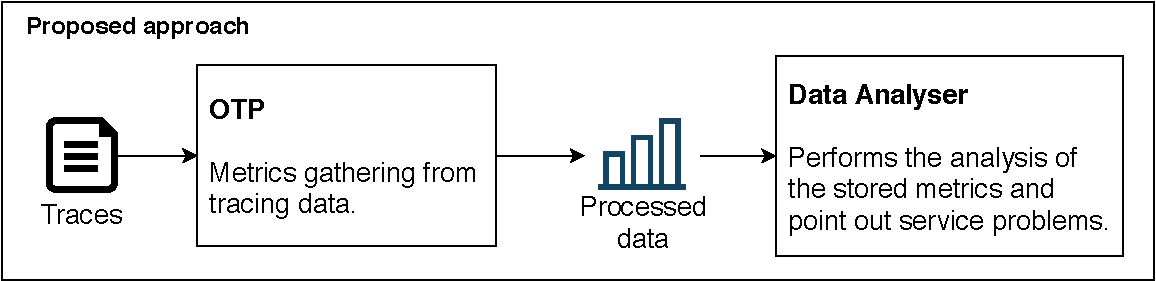
\includegraphics[width=1.00\textwidth]{images/proposed_solution.pdf}
    \caption{Proposed approach.}
    \label{fig:proposed_approach}
\end{figure}

Figure~\ref{fig:proposed_approach} shows the proposed process order for tracing data. We expect to have two main components, one for data extraction and another for data analysis. The input for each are tracing data and processed data from the first component respectively. The outcome is to answer the research questions defined in Section~\ref{sec:research_questions}~-~\nameref{sec:research_questions}.

Next Section~\ref{sec:functional_requirements}~-~\nameref{sec:functional_requirements} covers the functional requirements for this solution.

\section{Functional Requirements}
\label{sec:functional_requirements}

In software engineering, functional requirements defines the intended function of a system and its components. To present the functional requirements for our solution proposition, an id, the corresponding name and its priority are provided. The notation used in priority was based on the urgency that we expected from feature implementation. Three priority levels were used: High, Medium and Low. Therefore, the functional requirements for the proposed solution, sorted by priority levels, are presented in Table~\ref{table:functional_requirements_specification}.

\begin{table}[H]
    \caption{Functional requirements specification.}
    \label{table:functional_requirements_specification}
    \centering
    \begin{tabularx}{\linewidth} {
            |>{\hsize=0.10\hsize}X|
            >{\hsize=0.75\hsize}X|
            >{\hsize=0.15\hsize}X|}
        \cline{1-3}
         \textbf{ID}
         & \textbf{Name}
         & \textbf{Priority}                                                                                                                                                                                  \\ \hline \hline
         FR-1
         & The system must be able to ingest tracing data from a files or external distributed tracing tools.
         & High \\ \hline
         FR-2
         & The system must be able to retrieve service dependency graphs from distributed tracing tools.
         & High \\ \hline
         FR-3
         & The system must be able to store service dependency graphs in a graph database.
         & High \\ \hline
         FR-4
         & The system must be able to store time-series metrics extracted from tracing data in a time-series database.
         & High \\ \hline
         FR-5
         & The system must be able to extract the number of calls per service (total, incoming and outgoing) from tracing data.
         & Medium \\ \hline
         FR-6
         & The system must be able to extract the response time per service from tracing data.
         & Medium \\ \hline
         FR-7
         & The system must be able to generate request work-flow paths from tracing data.
         & Medium \\ \hline
         FR-8
         & The system must be able to calculate request ratio of success and error, for specific services, from tracing data.
         & Medium \\ \hline
         FR-9
         & The system must be able to calculate the degree (total, in and out) of services from service dependency graphs.
         & Medium \\ \hline
         FR-10
         & The system must be able to retrieve the difference between two service dependency graphs.
         & Medium \\ \hline
         FR-11
         & The system must be able to produce a report about spans structure using a defined OpenTracing structural schema.
         & Low \\ \hline
         FR-12
         & The system must be able to calculate the time coverage of traces in a given time-frame.
         & Low \\ \hline
         FR-13
         & The system must be able to identify regions of outliers presented in multiple time-series.
         & Low \\ \hline
    \end{tabularx}
\end{table}

Functional requirements defined in Table~\ref{sec:functional_requirements} were written based on defined research questions presented in Section~\ref{sec:research_questions}. These functional requirements can be grouped in three groups due to their priority levels. The first four (FR-1 to FR-4) are presented with high level of priority, because they represent the base functionality needed to implement the remaining requirements. The next eight functional requirements (FR-5 to FR-11), are time based metric extraction from tracing. The remaining three (FR-12 to FR-14) are related with trace testing and anomaly detection based in time-series thus the low priority.

Next Section~\ref{sec:quality_attributes}~-~\nameref{sec:quality_attributes} covers the proposed approach non-functional requirements.

\section{Quality Attributes}
\label{sec:quality_attributes}

Another important consideration, when designing a software system, is to specify all the quality attributes (also called non-functional requirements). These type of requirements are usually Architecturally Significant Requirements and are the ones that require more from software architect's attention, as they reflect directly all architecture decisions. To specify them, a representation called utility tree is often used. In this tree, the \gls{qa} are placed by an order of priority considering their impact for the architecture and for the business. The priority codification for the \gls{qa} is:
%  in order to consider the trade-offs and decide the weight of each in the produced architecture.

\begin{itemize}
    \item H. High
    \item M. Medium
    \item L. Low
\end{itemize}

To describe them properly, six important aspects must be included in \gls{qa} definition: \emph{stimulus source}, \emph{stimulus}, \emph{environment}, \emph{artefact}, \emph{response} and \emph{measure of the response}.

Figure~\ref{fig:utility_tree} contains all raised \gls{qa} for this proposed solution exposed in an utility tree structure, sorted alphabetically by their general \gls{qa} name, and after by the architectural impact pair (Architecture and Business).

\begin{figure}[H]
    \centering
    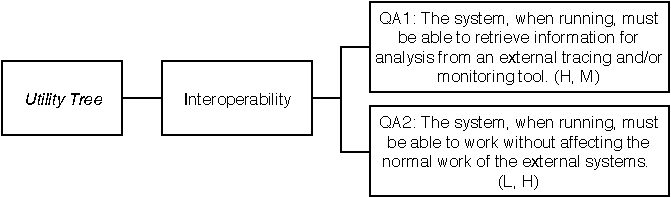
\includegraphics[width=1.00\textwidth]{images/utility_tree.pdf}
    \caption{\gls{qa} utility tree.}
    \label{fig:utility_tree}
\end{figure}

Figure~\ref{fig:utility_tree} shows us that only two Interoperability \gls{qa} were defined. An explanation for both is provided bellow:

\begin{itemize}
    \item[\textbf{QA1}] (Interoperability): Since the proposed solution must ingest tracing data. This information is usually found in distributed tracing tools already used by operators. To gather this information, access to an external distributed tracing tool is an important feature.As this is considered the starting point to obtain our data, we considered a Medium level for the architecture and a Low for the business.

    \item[\textbf{QA2}] (Interoperability): Since the proposed solution will be accessing an external distributed tracing system or outputs generated by it, all interactions with these systems must not cause conflicts. This is very important in the business perspective, because if our solution is not co-habitable with already used systems, it may be completely rejected. For the architectural perspective it does not represent a big impact, and therefore a Low level was assigned.

    %\item[\textbf{QA3}] (Performance): We defined this \gls{qa} taking into account the number of spans produced in an hour, by the system were we gathered our data. As it produces approximately 200.000 spans in an hour, and to ease our research work when using the tool, we decided to set the target for our solution as 1.000.000 spans in about a minute. This \gls{qa} will have an high architectural impact, as it can define a certain technology for graph processing. For the business perspective, we considered a Medium level, as it presents some interest.

    %\item[\textbf{QA4}] (Scalability): Due to the amount of data needed to process and store over time, our system has to be able to store the data into multiple machines because it may start running out of space. We decided to give a medium level of architectural impact as it can change the solution in terms of storage components. For the business this has an high impact, as it need more machines to run the solution if this \gls{qa} is fully considered against the remaining.

    %\item[\textbf{QA5}] (Traceability): This \gls{qa} was considered due to the simple fact that we need to bee able to see what's the system is doing, when it's processing the data. For this \gls{qa} we decided to give low levels for both architecture and business, as it does not represent relevance to any of them.

    %\item[\textbf{QA6}] (Testability): As the system will be analysing external systems, we need to be sure that it analyses it in a correct way, and to be sure of this we need to test our solution. We considered a medium level for the architectural impact for this \gls{qa}, because its implementation needs to analyse some components from within the system. For the business we considered a low level, because the main interest to test the system is ours in order check if it is working correctly.
\end{itemize}

\section{Technical Restrictions}
\label{sec:technical_restrictions}

In this Section, technical restrictions considered in proposed solution are presented.

In software engineering, after specifying functional and non-functional requirements for a solution, comes the specification of business restrictions, however, in this project none were raised due to the fact that this work is focused on exploration and research.
%, and that there isn't any formal client defined.

To define the technical restrictions, we used an id and its corresponding description. Table~\ref{table:technical_restrictions_specification} presents the technical restrictions considered for the proposed solution.

\begin{table}[H]
    \caption{Technical restrictions specification.}
    \label{table:technical_restrictions_specification}
    \centering
    \begin{tabularx}{\linewidth} {
        |>{\hsize=0.25\hsize}X|
        >{\hsize=0.75\hsize}X| }
        \cline{1-2}
        \textbf{ID}
         & \textbf{Description}                    \\ \hline
        TR-1
         & Use \emph{OpenTSDB} as a Time-Series database. \\ \hline
    \end{tabularx}
\end{table}

Table~\ref{table:technical_restrictions_specification} shows that we have raised only one technical restriction. This technical restriction was considered because Professor Jorge Cardoso, acting as a client for this solution demanded it. \emph{OpenTSDB} is the database that they are currently using in their projects at Huawei Research Center. This restriction will ease their work to introduce changes if needed.
%However, this project does not have a concrete and formally defined client, it is good to use a technology used by the people that will use the tool to ease their work and possibly introduce changes.

\section{Architecture}
\label{sec:architecture}

In this Section, the architecture is presented based on all previous topics with resource to the defined Simon Brown’s C4 Model~\cite{simon_browns_c4_model}. This approach of defining an architecture uses four diagrams: \emph{1 - Context Diagram}, \emph{2 - Container Diagram}, \emph{3 - Component Diagram} and \emph{4 - Code Diagram}. To define the architecture for our solution, only the first three representations were considered. Every representation will be exposed with a explanation of the decisions taken to draw each diagram. After presenting the representations and the corresponding explanations, we will cycle thought all architectural drivers: \gls{qa}, bussines and technical restrictions, in order to explain where they are reflected and the considerations taken to produce this architecture.

\subsection{Context Diagram}
\label{subsec:context_diagram}

In this Subsection the context diagram is presented. This diagram allows us to see ``the big picture'' of the overall system as it represents the system as a ``big box'' and the corresponding interactions with users and external software systems. Figure~\ref{fig:context_diagram} presents the context diagram for this solution.

\begin{figure}[H]
    \centering
    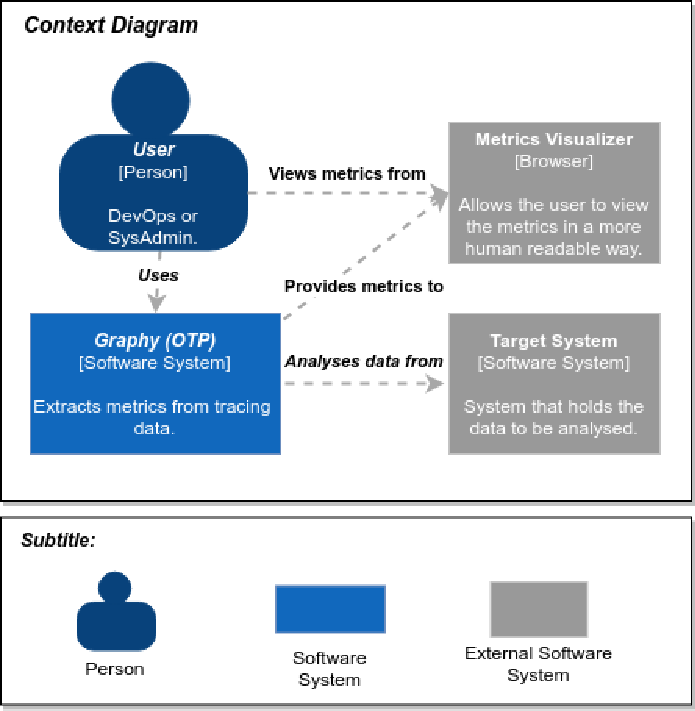
\includegraphics[width=1.0\textwidth]{images/context_diagram.pdf}
    \caption{Context diagram.}
    \label{fig:context_diagram}
\end{figure}

From Figure~\ref{fig:context_diagram}, we can see that our solution, named \emph{Graphy \gls{otp}}, receives interactions from users, as it need someone to start the whole process. This piece of software analyses data from an external target system that holds the tracing information and consequently, provides extracted metrics to an external metrics visualizer component. Users can view extracted metrics from this last component. Also, reports are produced and stored within our solution, when it performs tracing analysis. 

\subsection{Container Diagram}
\label{subsec:container_diagram}

The container diagram is presented in this Subsection. This type of diagram allows us to ``zoom-in'' in the context diagram, and get a new overview of our solution. Therefore, in this diagram we are able to see a high-level shape of the software architecture and how responsibilities are distributed across containers. Figure~\ref{fig:container_diagram} presents the container diagram for our proposed solution.

\begin{figure}[H]
    \centering
    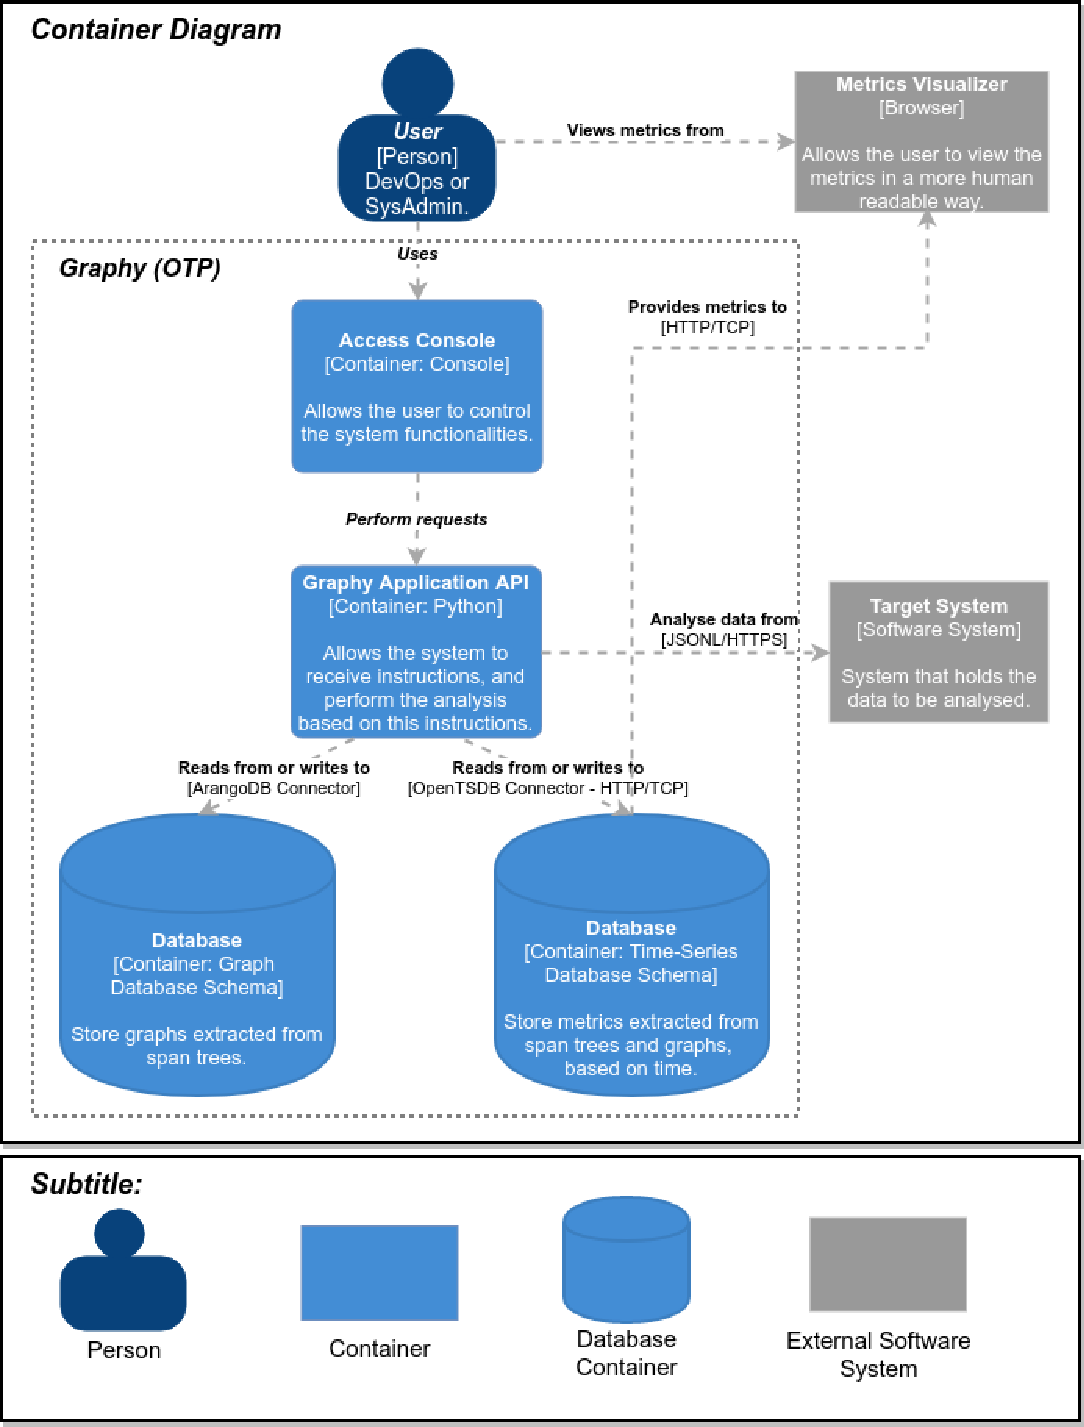
\includegraphics[width=1.00\textwidth]{images/container_diagram.pdf}
    \caption{Container diagram.}
    \label{fig:container_diagram}
\end{figure}

\newpage

Figure~\ref{fig:container_diagram} contains the main containers involved in our solution. The first one, from top to bottom, is the \emph{Access Console} and this container was considered as it is needed for the user to be able interact with the \emph{Graphy \gls{api}}. This last one controls the entire OpenTracing system, uses a communication protocol to retrieve tracing information from external target system, and two databases to store the information resulted from processing tracing data -- a \gls{gdb} and a \gls{tsdb}. The second database provides metrics to be visualized in an external metrics visualizer system.

\subsection{Component Diagram}
\label{subsec:component_diagram}

This Subsection contains the last diagram, the component diagram. This type of diagram gives a more deeper vision about the system, and therefore, it reveals the main components. Figure~\ref{fig:component_diagram} presents the component diagram for this solution.

\begin{figure}[]
    \centering
    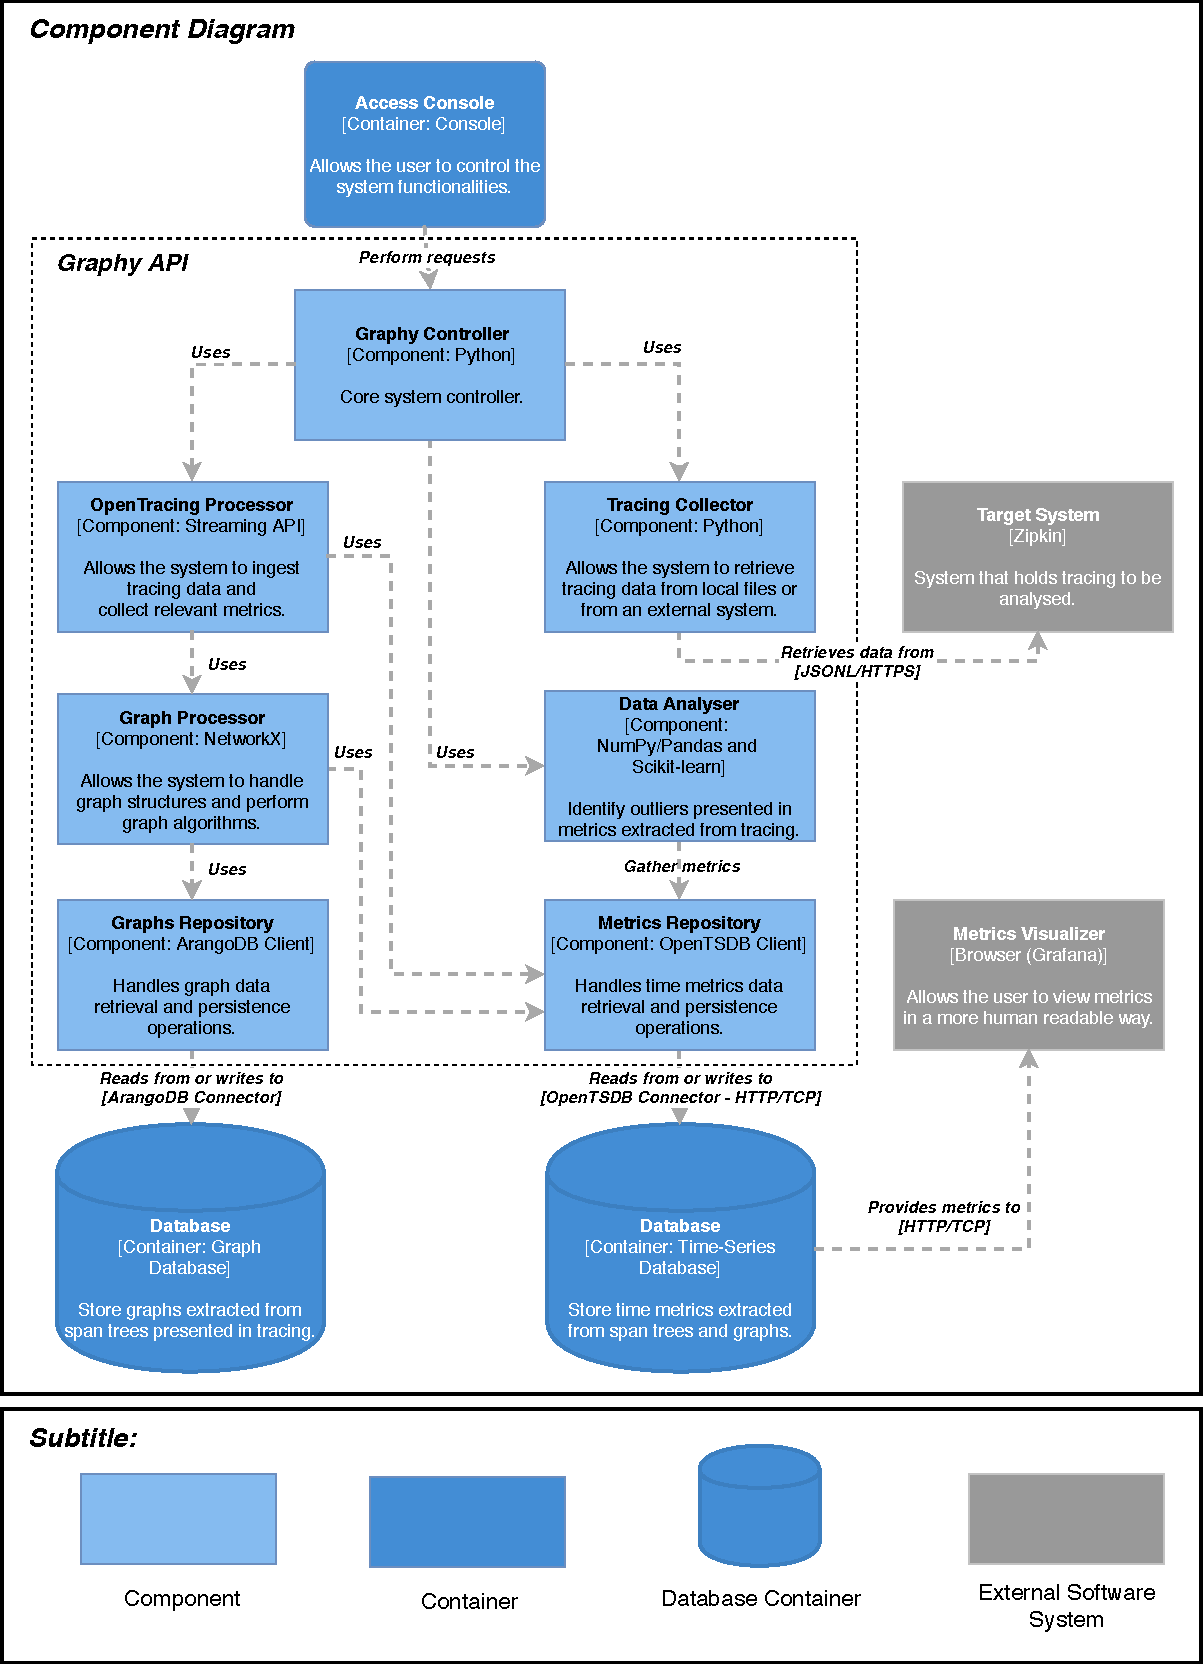
\includegraphics[width=1.00\textwidth]{images/component_diagram.pdf}
    \caption{Component diagram.}
    \label{fig:component_diagram}
\end{figure}

Figure~\ref{fig:component_diagram} provides us with a lower level visualization of \emph{Graphy API} container composed by eight components. At its core we have \emph{Graphy Controller}, a component with the responsibility of receiving requests from the user through \emph{Access Console} and control \emph{OpenTracing Processor}, \emph{Tracing Collector} and \emph{Data Analyser} components. The first one has the objective of mapping tracing data, span trees and service dependency graphs instantiation into memory. The second one collects tracing, the information that feeds this entire application, from local files or from external systems, e.g., \emph{Zipkin}. The last one, \emph{Data Analyser}, identifies outliers presented in time-series metrics extracted from tracing, allowing our solution to detect anomalous services presented in distributed systems. \emph{Graph Processor} is the component for graphs handling, thus it has the capability of performing operations over graphs, e.g., subtract one graph from another, extract node degrees and count connections between nodes. The remaining components, \emph{Graphs Repository} and \emph{Metrics Repository}, are used to map graphs and time-series metrics, respectively, into and from their corresponding databases.

To check the architecture produced, we will now cycle between both \gls{qa} and check were they are reflected in the architecture presented for this solution, explaining the trade-off involved and what were our considerations about each one.

\gls{qa}1 and \gls{qa}2 are satisfied by the fact that the system is able to collect data from an external system. Using a communication protocol where data is exchanged thought \gls{http} and exposed \gls{api}, allows to externally request little chucks of data from target systems without interfering with their normal function.

%\gls{qa}3 is satisfied when we decide to use NetworkX as the technology to process our graphs. This technology does not scale horizontally, however it has a very decent performance and it's able to retrieve a certain measure of a graph with about 100.000 nodes, in near 15 seconds\cite{networkx_speed}. From 1.000.000 spans, in normal conditions, we will never be able to get a graph of this kind of size, as with our experiments, with 100.000 spans we were able to get a graph of almost 20 nodes, and with 200.000 spans we were able to get a graph of almost 30 nodes. In the end, we are considering this time and span quantity to be sure that our tool will give us good times and ease our work of performing the research and implementation of this kind of tool.

%\gls{qa}4 is satisfied because we decided to use two databases that are scalable horizontally by design, the ArangoDb for a \gls{gdb} and the \emph{OpenTSDB} for a \gls{tsdb}, both presented in the \ref{subsec:graph_database_tools} and \ref{subsec:time_series_database_tools} subsections respectively. In the end, this \gls{qa} can not be fully satisfied because we can not scale our system entirely, due to the fact of the technology that we chose to perform the graph processing. However, we have chosen this technology because it can perform much more graph algorithms, as we can see in the figure \ref{fig:graph_manipulation_and_performance_tools_diagram_comparison}, and this is much more relevant for our main purpose.

%\gls{qa}5 is satisfied by the existence of the component \textit{Logging Component}, that allows the system to perform logging of relevant information. For the technology here, we decided to use click-log\cite{click_log_doc}, a python library used for logging purposes as it has all the main capabilities needed here to perform the logging.

%\gls{qa}6, like the previous one is satisfied by the existence of a certain component, the \textit{Testing Component}, which implements all the capabilities and functionalities to perform tests and check if the systems is working correctly.

Finally, for the only technical restriction raised, we can see that it is satisfied by the usage of \emph{OpenTSDB} as the main \gls{tsdb} for our solution.

This solution does not have many architectural drivers: quality attributes, business constraints and technical restrictions, due to being a prototype. The main objective is to produce a solution capable of explore tracing data allowing us to conduct a research about what we can do with tracing, therefore it does not have many architectural constraints. Nevertheless, with the presentation of these four sections, we conclude that our solution satisfies all the architectural drivers, and therefore, we may claim that the proposed architecture fits our needs as a solution.

Next Chapter,~\ref{chap:implementation_process}~-~\nameref{chap:implementation_process}, covers the implementation of the solution presented in the current chapter. All implemented algorithms and technical decisions are discussed and explained in detail.

\checkoddpage
\ifthenelse{\boolean{oddpage}}
{ % Odd page
    \newpage
    \blankpage}
{ % Even page
}